% -------------------------------------------------

\documentclass[a4,12pt]{article}

%==============================================================================
%% Packages and Command Setting

\usepackage{geometry}
\usepackage{svg}
\usepackage{minted}
\usepackage{enumitem}
\usepackage{hyperref}
\usepackage{graphicx}
\usepackage{biblatex}
\usepackage{caption}
\usepackage{subcaption}
\usepackage[compact]{titlesec}

\definecolor{bg}{rgb}{0.95,0.95,0.95}

\immediate\write18{[[ ! -f "public/logo-black.svg" ]] ||
sed 's/00BEC9/1c1c1c/' public/logo.svg >public/logo-black.svg}

\addbibresource{references.bib}

\titlespacing\section{0pt}{8pt plus 4pt minus 2pt}{0pt plus 2pt minus 2pt}
\titlespacing\subsection{0pt}{8pt plus 4pt minus 2pt}{0pt plus 2pt minus 2pt}
\titlespacing\subsubsection{0pt}{8pt plus 4pt minus 2pt}{0pt plus 2pt minus 2pt}
\setlength{\parindent}{0pt}

\title{%
    
\includegraphics{public/CompSci_mono}\\[\bigskipamount]
    {\Large Human Centered Security (M) Coursework \par}
    \vskip 1em%
    \includesvg[width=130pt]{public/logo-black.svg}\par
    \vskip 1em%
    {\LARGE Authentica \par}
    \large
}

\author{%
    Anna Berry (2373329)\\
    Hector Jones (2375347)\\
    Inesh Bose (2504266)\\
    Marc Auf der Heyde (2326744)\\
    Stephen Connolly (2389475)
}

\date{}

\begin{document}

\onecolumn
\maketitle
\vfill

%===============================================================================
% Introduction

\section*{Introduction}

The motivation behind the Authentica website is the recent increase in online document usage during the pandemic. Some of these online documents are public and require signatures to authenticate the owner of the document.

Currently the existing methods of signing a document include, the use of “print name”, which involves typing your name in a document. This is a fairly accepted form of signature for online documents, but nothing about it is secure and authentic as you can type in anyone's name. A digital signature can also be generated using a Handwriting Font but these are also insecure as they can easily be copied. An alternative option is attaching an image of your signature, but that image asset, can easily be downloaded and reused, similarly to the handwriting font signature. Finally, you could just print out the document, sign it, scan it, and put it online but that is not convenient to users, and so they would look for easier lazier alternatives.

Authentica was developed to mitigate the risks of current digital signing methods and allow for seamless signatures in the digital world. This report will discuss the concept behind Authentica, how it was implemented, evaluated and what the results of our evaluation showed about users and their security practices when it comes to online signatures.


%===============================================================================
% Concept and Implementation

\section*{Concept and Implementation}

Authentica is a novel digital signature system, which uses public-key cryptography to allow users to sign digital documents, thereby verifying them.

Every account made in Authentica has a public-private key pair created for it. The Elliptic npm package \cite{elliptic} was used to generate a public and private key upon a user registering at Authentica.

When a  digital document is signed, a hash is generated from the document name and the current timestamp using the \texttt{js-sha3} npm package \cite{sha}. This document is then signed using the user's private key to produce a document signature and message hash. The document key is not a cryptographic key like the public-private key pair, it is a unique identifier encrypted by the private key of the public-private key pair.

To verify another persons signature the Document key is shared alongside the digital document and the public key of the user who shared the document are used to try and verify that the private key of the user who shared the document, was used to generate the document key. The implementation can be viewed in the Appendix \ref{fig:signature}.

\subsection*{Technology \& Stack}

Next.js is an extension of the React framework, it is a commonly used frontend library using a component based system to build user interfaces and to provide server-side rendering, along with an API. \cite{nextjsclock}. A benefit of using Next.js was that it allowed the team to easily deploy our system on Vercel \cite{authenticavercel} (as it is the company that developed Next.js \cite{vercel}) directly from our repository \cite{authenticarepo}.

The backend of the system consisted of Prisma ORM (object-relation mapper) with SQLite as our database. The requirements of our schema and relationships were quite simple, having only a user and document model in a one-to-many relationship, as shown in Figure \ref{fig:schema}. It is for this reason we believed it would be in our best interests to have the high level abstraction provided by Prisma \cite{prismaorm}, as we did not require complex database queries.

The query language GraphQL was used alongside Next.js and Prisma ORM. This was chosen over a normal REST API because GraphQL is strongly typed, which compliments our decision to use Typescript, so that at all times we know what form data takes and also what is available to us \cite{stablekernel}. When making HTTP requests using a REST API, responses usually contain more data than is actually required, whereas using GraphQL queries, only the specified data is returned \cite{javatpoint}.

The user interface was created using Geist UI \cite{geistui}. This design system was chosen as it was adopted by our inspiration project, Krates \cite{krates}, which helped us conceptualise Authentica as an application based on Krates' design. We believed it was appropriate to use the minimalist and visually pleasing design, to facilitate usability and ensure minimal user frustration when interacting with our application.

\subsection*{Final Implementation}

The final implementation allowed users to view a tutorial, login and register for an Authentica account, sign documents and create a shareable URL that can verify the document. The key features of the final implementation are shown in Figure \ref{fig:model} and are summarised below:

\begin{itemize}[leftmargin=*, label={}]
    \setlength\itemsep{0em}
    \item \textbf{Tutorial:} Users can press on the 'Learn More' button to be taken to a short introduction about Authentica, how it works and what they can use it for.
    \item \textbf{Register and Login:} Users without an account are able to register an account with Authentica, once registered they are automatically logged in to use the system. Otherwise if they have an account they can visit the login form for access.
    \item \textbf{Sign a Document:} Users are able to input the name of their document, and submit this to be signed, they will receive a display of the filename along with a shareable URL and the equivalent hash.
    \item \textbf{Delete a Document:} Finally, a user can delete a document, removing it from their account and deleting the linked signature.
\end{itemize}


\begin{figure}[htb]
    \centering
    \begin{subfigure}[b]{0.3\textwidth}
        \centering
        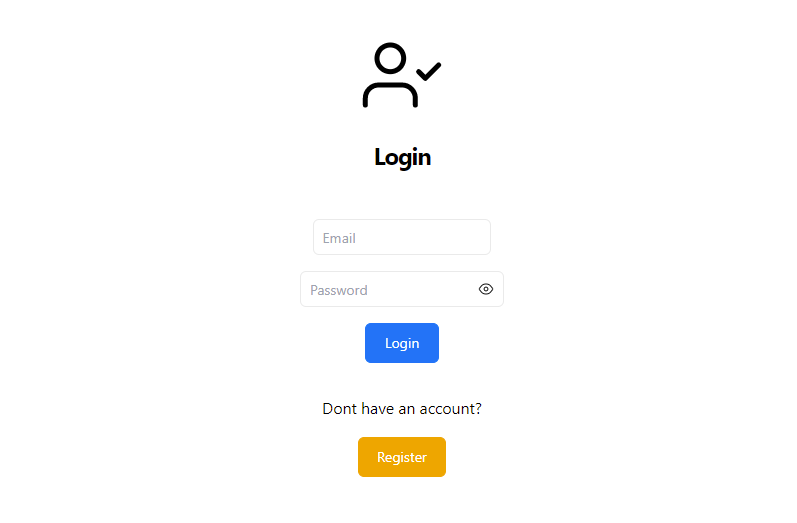
\includegraphics[width=\textwidth]{public/login.png}
        \caption{User logs in}
    \end{subfigure}
    \hfill
    \begin{subfigure}[b]{0.3\textwidth}
        \centering
        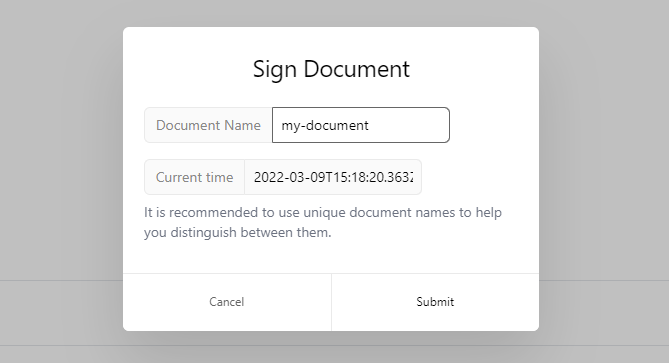
\includegraphics[width=\textwidth]{public/sign_form.png}
        \caption{Once logged in, users can sign documents}
    \end{subfigure}
    \hfill
    \begin{subfigure}[b]{0.3\textwidth}
        \centering
        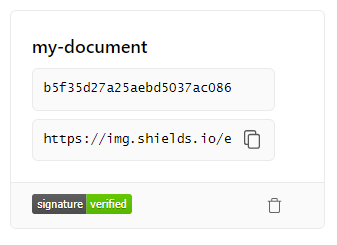
\includegraphics[width=\textwidth]{public/doc_card.png}
        \caption{A URL is then produced, this can be shared to verify the document}
    \end{subfigure}
    \caption{Implementation of Log in, Sign Document and Sharable signature URL}
    \label{fig:model}
\end{figure}

%===============================================================================
% Evaluation

\section*{Evaluation}

\begin{itemize}[leftmargin=*, label={}]

\setlength\itemsep{0em}

\item \textbf{Study Goal:} To evaluate the usability and user experience of our novel electronic signature system.

\item \textbf{Threat Model:} In the threat model for our user study, we focus on usability failures which might be caused by the system. The primary threat in this model is therefore the user themselves, who might undergo insecure operations due to a fundamental lack of understanding.

\item \textbf{Measures (Dependent Variables):} The study will measure the system usability; the system usability scale survey will be administered to participants upon completing the evaluation, to measure a definitive score for the usability of the system. Alongside the System Usability survey, we will administer the user experience questionnaire for products to evaluate the overall user experience. The survey was administered through a google form \cite{gform}. % The Google Form for the System Usability Survey and the user experience questionnaire can be found here.

\item \textbf{Independent Variables:} The user study will consist of one independent variable, the digital signature system, Authentica. This will be evaluated in terms of usability and user experience.

\item \textbf{Design Structure:} The study will take on a within-subject design.

\item \textbf{General Procedure:} This study will consist of several digital document signing tasks, which will be observed through in-person cognitive walkthroughs. Following the completion of the tasks, users will be asked to fill out a system usability scale to evaluate the overall usability of Authentica. Before beginning the study, each participant will be required to give explicit consent before proceeding, as in line with the ethics requirements. Participants will also be debriefed after the study is over, and have the express right to end the study at any point in time. All data, both quantitative and qualitative will be stored anonymously with identifying attributes removed before publishing.

\item \textbf{User Tasks:} Participants were asked to complete the a set of tasks and were encouraged to think-aloud,explaining their process, as they completed them. Participants were asked to ; create and account, sign a dummy document, view signed documents, share their verified document and finally delete a document.

%The participant should create an account at Authentica.The participant should sign a dummy document available on the test machine (the experimenter may give help if the OS being used is not the participant’s native OS).The participant should view their previously signed documents.The participant should find the available signature URL generated by signing the document. This can be shared with other individuals and the document to show a verified signature badge. Save this link to paste in the field below.The participant should delete a previously signed document from their list.

\item \textbf{Data Analysis Plan:} The System Usability Score will be calculated from the administered System Usability Surveys, following the completion of the study. The User Experience Questionnaire will be analyzed using the corresponding spreadsheets found on the UEQ website \cite{ueq}. The qualitative data collected through the cognitive-walkthroughs will be coded and processed.

\end{itemize}

% Discussion: a) summarize the results, then b) discuss what can be learnt from the results and c) reflect on the encountered challenges (rather than focusing on technical challenges, focus on conceptual usability and security challenges that are relevant to researchers and practitioners).

\section*{Results \& Discussion}

Twelve participants evaluated Authentica.  Ten participants were in the age range 20-25 and two participants in the age range 60-65, 42\% of participants were female and 58\% male.
Following the completion of our participant evaluation, we proceeded to analyse the data captured through the administered questionnaires to determine the overall usability and user experience of our designed system.

The results of the System Usability Survey (SUS) showed definitively that the overall usability of Authentica is above average. Our calculated mean SUS score is 83, and the SUS guidelines determine that any achieved score over 68 can be counted as above average. All users had a SUS score of above 68 as shown in Figure \ref{fig:SUS_UEQ_Mean_Variance}. SUS Scores closer to this measure should be normalized to return a percentile ranking, but our results did not suffer from this.

As a result, this System Usability Score generally indicates that a system is usable as a whole, and likely not suffering from any serious caveats which might be inhibiting overall usability. Though it does not eliminate such caveats entirely, it does support such a hypothesis.

\begin{figure}[htb]
    \centering
    % \begin{subfigure}[b]{0.6\textwidth}
    %     \centering
    %     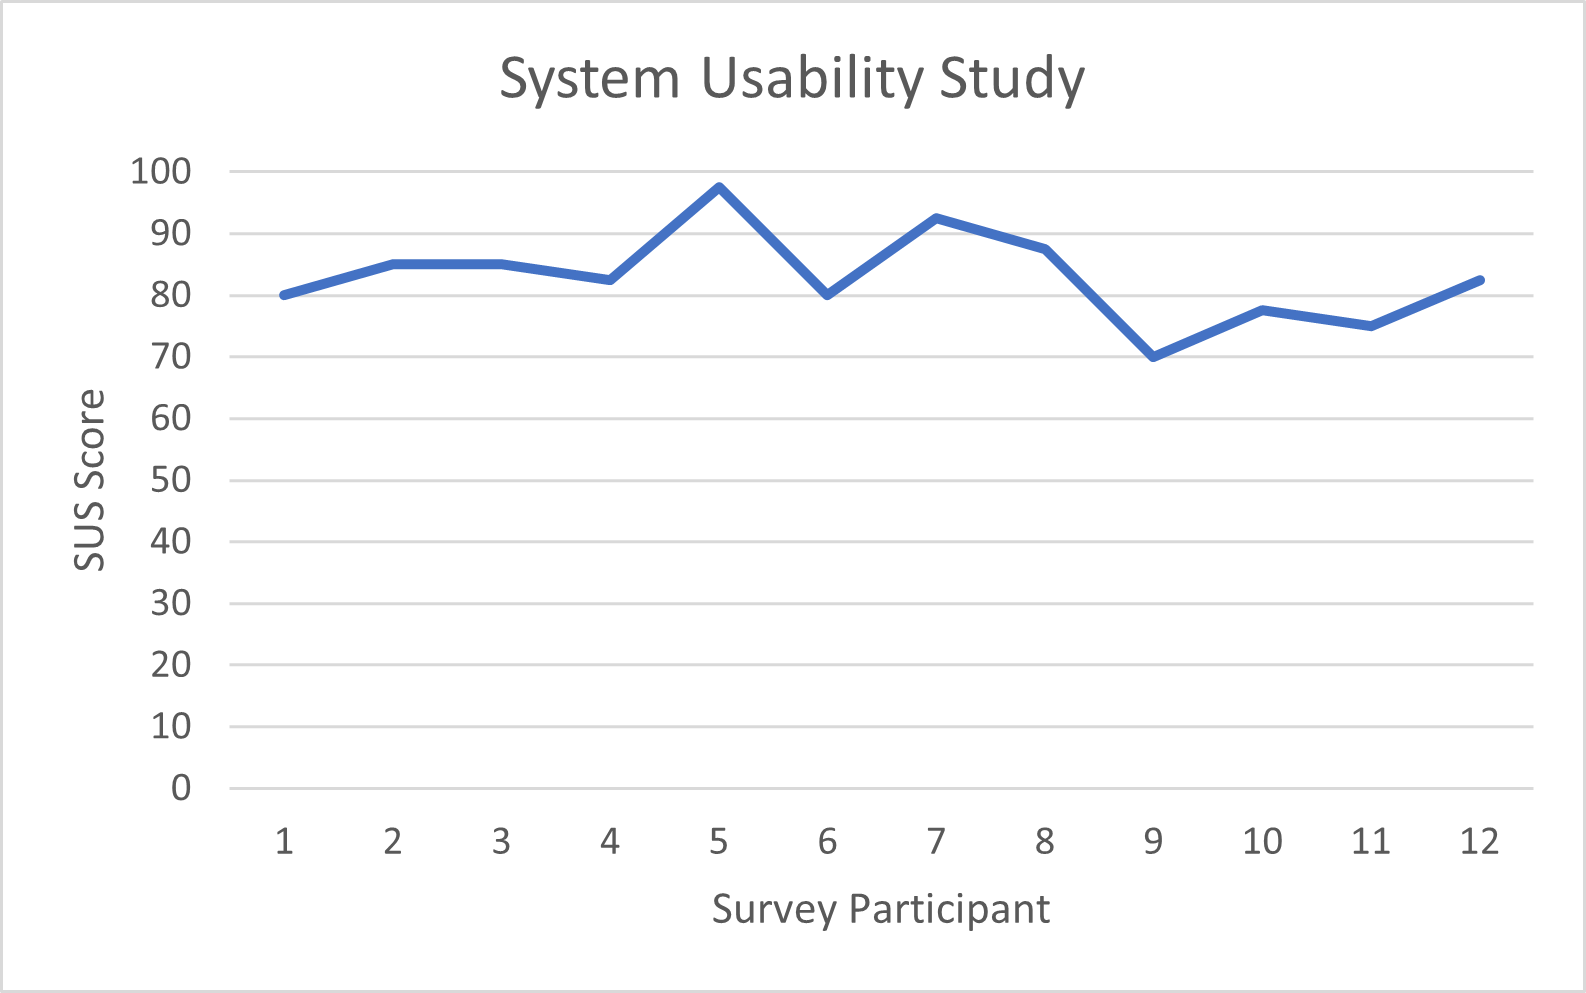
\includegraphics{public/SUS.png}
    %     \caption{System Usability Score}
    % \end{subfigure}
    % \hfill
    % \begin{subfigure}[b]{0.3\textwidth}
    %     \centering
    %     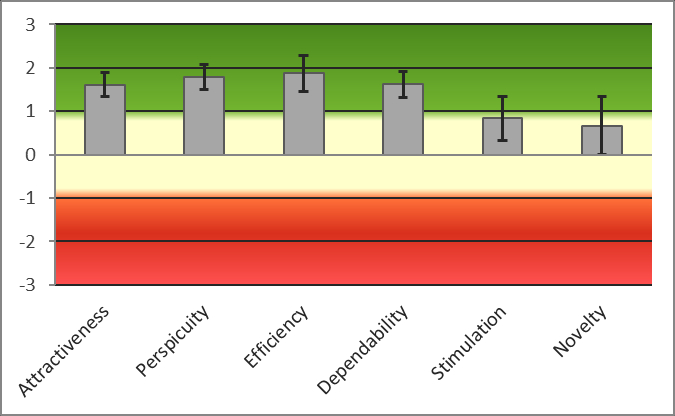
\includegraphics{public/results/UEQ_Scales_Mean.jpg}
    %     \caption{UEQ Mean and Variance Graph}
    % \end{subfigure}
    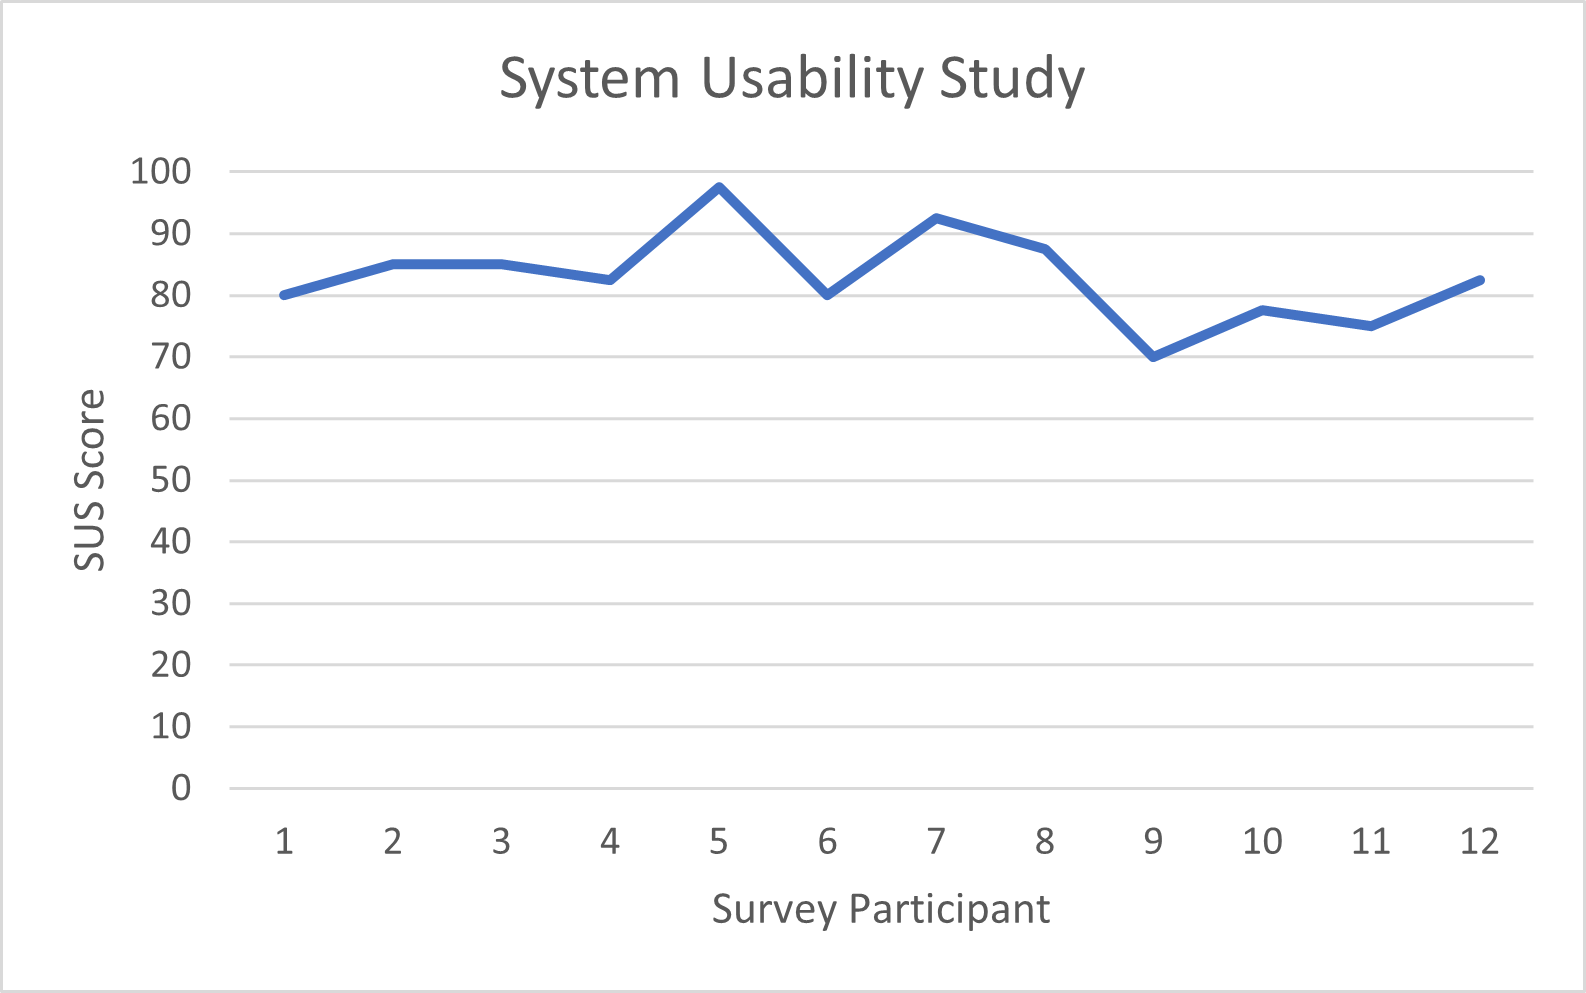
\includegraphics[scale=0.6]{public/SUS.png}
    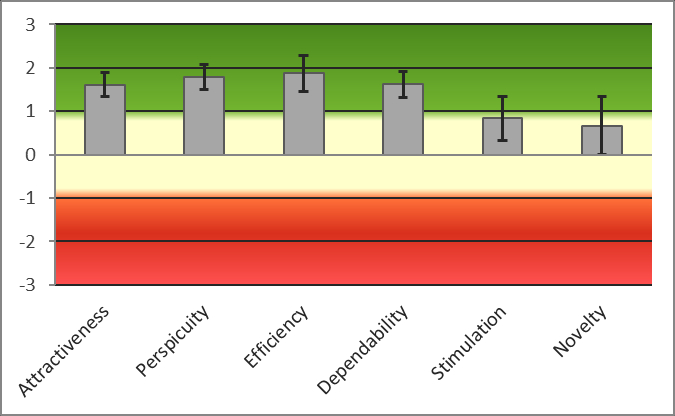
\includegraphics[scale=0.3]{public/results/UEQ_Scales_Mean.jpg}
    \caption{System Usability Score (Left) and UEQ Mean and Variance Graph (Right).}
    \label{fig:SUS_UEQ_Mean_Variance}
\end{figure}

The results of the User Experience Questionnaire were analysed next using the analysis tool distributed by the creators of the UEQ \cite{ueq}. The analysis tool used in the UEQ analysis is different from the analysis performed on System Usability Scores. The analysis tool provides scores for six different user experience characteristics, namely, attractiveness, perspicuity, efficiency, dependability, stimulation and novelty. The resulting graph depicting scores for each category in the range -3 (horribly bad) to +3 (extremely good), can be seen below. A corresponding table with the means and variance for each category can be found in the Appendix section.

To give a clearer indication of what such scores mean, the analysis tool supplies a benchmark data set of UEQ results, which can be used to infer the degree of goodness of an overall user experience based on each of the User Experience categories. % Table \ref{fig:UEQ_Benchmark_Table} shows how the Authentica User Experience fairs against results from the benchmark data set. A graph depicting the values from the table can be found in Appendix section B.

The comparative table is measured in bad \textrightarrow below average \textrightarrow above average \textrightarrow good \textrightarrow excellent. As can be seen in Figure \ref{fig:SUS_UEQ_Mean_Variance}, Authentica performed very well in 4/6 of the User Experience categories, notably in attractiveness, perspicuity, efficiency and dependability, the table can be found in the Appendix Table \ref{fig:UEQ_Benchmark_Table}. Interestingly enough, users found their Authentica User Experience to be below average in a stimulating sense and below average in a sense of novelty. This can be at least in part explained due to the technical expertise of the participants evaluated. Without having an in-depth understanding of the importance of online document authentication, Authentica can only be so stimulating. This is a particular area in which there is much room for improvement. Future work should take into consideration how a system such as Authentica can be made stimulating for everyday users.

The observations from the cognitive walk through and the administered survey also helped give an understanding of what users thought of Authentica. From user observations, all users managed to complete all tasks with little difficulty showing that the document signing process was intuitive. User comments also found users enjoyed the website design. Some aspects of Authentica confused users given that almost all users did not navigate to the Tutorial page and those who did did not take the time to read it all. Users experienced confusion with how Authentica worked and why they were sharing a URL to share their signature. Users also struggled to identify the cards used to represent documents as their signed documents, expecting to see and view a full document. the lack of clear headings and viewing of the tutorial led to users not having a full understanding of how Authentica worked.

% \begin{figure} %can make smaller
%     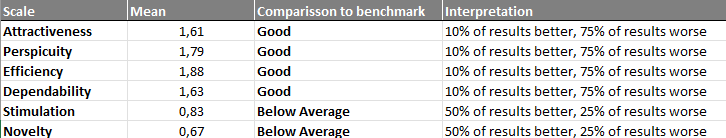
\includegraphics[scale=0.8]{public/results/UEQ_Benchmark_Table.png}
%     \centering
%     \caption{UEQ Benchmark Table}
%     \label{fig:UEQ_Benchmark_Table}
% \end{figure}

%==============================================================================
% Conclusion and Future Work

\section*{Conclusion and Future Work}
Overall the Authentica website we produced was successful in receiving good usability feedback. Although users encountered some problems, with a little more time further refinements could be made to allow Authentica to meet all of the users needs.

The SUS and UEQ results show users found Authentica to be usable. Authentica had a SUS score of 83 which is above average and shows that the system is usable. The UEQ survey showed that users rated Authentica highly in attractiveness, perspicuity, efficiency and dependability. The only places Authentica fell short was in being stimulating and its novelty.

A major struggle in security is getting users to read and understand what it means, although we attempted to educate our users on the details of how the document signing is working in the background, we failed to do this in clearly signposted a simple enough way. Although users were able to navigate and use our website effectively it is not clear if they always knew why they were doing each step, or how the website would be useful to them in the future.

The time constraint limited further development on the UI/UX side. If Authentica was to be further developed it would be important to take into account the issues we discovered from our User Study. It would be important to implement a tutorial that was simple to understand while still being informative. The tutorial page could be updated to include less daunting language, such as keys and encryption, and explain Authentica in a way some one less familiar with security could understand. Another way the tutorial could be modified is to include a walk-through for users when they first register explaining why they are carrying out steps. Clearer headers on the signed document section and tool-tips could also be implemented offering quick reminders of functionality.

In addition to fixing the issues we discovered, Authentica could also have additional features added. The ability to upload documents and have the signature linked to the document, similar to Eversign \cite{eversign}. The signature link could also be integrated into the document so you can send and receive a document that is signed and simply click the link to verify it. Authentica could also have integration with GitHub authentication. Visualising and playing with the API data could have been easier with a browsable API like the one in Django REST Framework \cite{DRF}. This would have allowed for keys to be directly inputted into the database and data being viewed instead of relying on URLs.

%==============================================================================
%% References & Appendix

\newpage
\printbibliography

\appendix

\newpage
\newgeometry{bottom=20mm}
\section{Code Appendix}

\begin{figure}[h]
\centering
\begin{minted}[bgcolor=bg]{psql}
model User {
  id        Int        @id @default(autoincrement())
  email     String     @unique
  password  String
  pubkey    String
  privkey   String
  documents Document[]
}

model Document {
  id        String     @id
  user      User       @relation(...)
  userId    Int
  signature String
}
\end{minted}
\caption{Schema definition in \href{https://github.com/ineshbose/authentica/blob/9ceaf3575cc26b7bb5be035e24d779237d829de4/prisma/schema.prisma\#L10}{\texttt{prisma/schema.prisma}}}
\label{fig:schema}
\end{figure}

\begin{figure}[h]
\centering
\begin{minted}[bgcolor=bg]{typescript}
const signDoc = (privKey, name, time) =>
  JSON.stringify({
    ...ec.sign(
      sha3.keccak256(`${name}${time}`),
      privKey, 'hex', { canonical: true },
    ), name,
  });

const verifyDoc = (pubKey, msgHash, signature) =>
  ec.verify(msgHash, signature, pubKey, 'hex');
\end{minted}
\caption{Pseudo Function definitions for signature handling in \href{https://github.com/ineshbose/authentica/blob/9ceaf3575cc26b7bb5be035e24d779237d829de4/lib/keygen.ts\#L17}{\texttt{lib/keygen.ts}}}
\label{fig:signature}
\end{figure}

\newpage
\section{Result Appendix}

\begin{table}[htb]
    \centering
    \begin{tabular}{l|l|l}
    \multicolumn{3}{l}{UEQ Scales (Mean and Variance)} \\ \hline
    Attractiveness        & 1,6111        & 0,24       \\
    Perspicuity           & 1,7972        & 0,27       \\
    Efficiency            & 1,875         & 0,53       \\
    Dependability         & 1,625         & 0,28       \\
    Simulation            & 0,833         & 0,78       \\
    Novelty               & 0,667         & 1,38
    \end{tabular}
    \caption{UEQ Mean and Variance Table}
\end{table}

% \begin{figure} %can make smaller
%     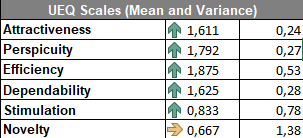
\includegraphics[]{public/results/UEQ_Scales_Mean_and_Variance.png}
%     \centering
%     \caption{UEQ Mean and Variance Table}
%     \label{fig:UEQ_Mean_Variance}
% \end{figure}

\begin{table}[htb]
    \centering
    \addtolength{\leftskip} {-2cm}
    \addtolength{\rightskip}{-2cm}
    \begin{tabular}{l|l|l|l}
    Scale & Mean & Comparison to benchmark & Interpretation
    \\ \hline
    Attractiveness & 1,61 & Good                    & 10\% of the results better, 75\% of results worse \\
    Perspicuity    & 1,79 & Good                    & 10\% of the results better, 75\% of results worse \\
    Efficiency     & 1,88 & Good                    & 10\% of the results better, 75\% of results worse \\
    Dependability  & 1,63 & Good                    & 10\% of the results better, 75\% of results worse \\
    Simulation     & 0,83 & Below Average           & 50\% of the results better, 25\% of results worse \\
    Novelty        & 0,67 & Below Average           & 50\% of the results better, 25\% of results worse
    \end{tabular}
    \caption{UEQ Benchmark Table}
    \label{fig:UEQ_Benchmark_Table}
\end{table}

\begin{figure}[htb]
    \centering
    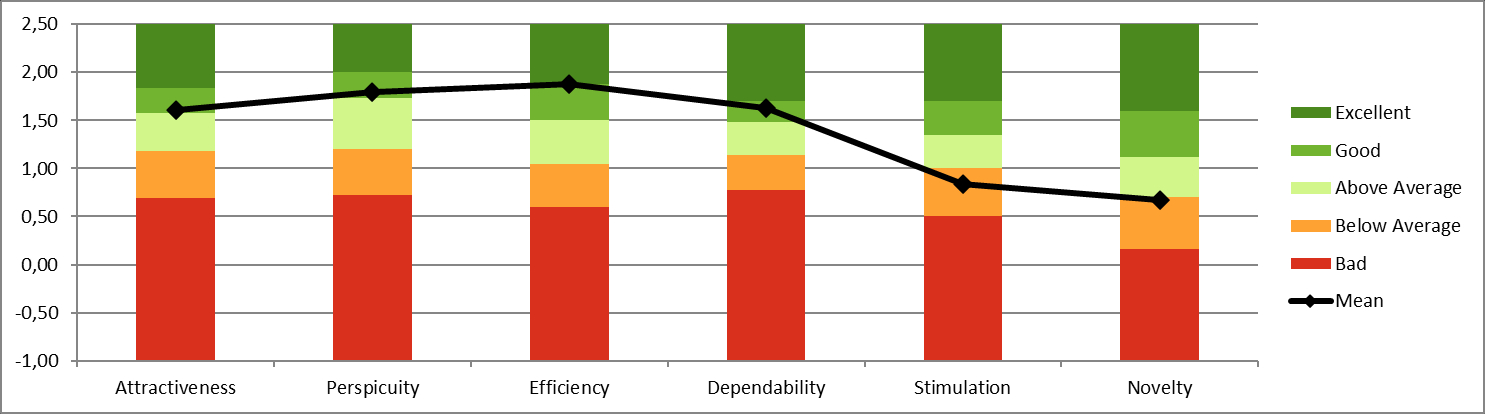
\includegraphics[scale=0.3]{public/results/UEQ_Benchmark_Graph.jpg}
    \caption{UEQ Benchmark Graph}
\end{figure}

\end{document}
